\documentclass[a4paper,12pt,amsmath,amssymb,aps]{article}
\usepackage[utf8]{inputenc}
\usepackage[T1]{fontenc}

% Mathematics
\usepackage{amsmath,amssymb,bm,mathtools}
\usepackage{gensymb}

% Figures
\usepackage{graphicx}
\usepackage{float}

% About the document
\title{
	Numerical Implementation of\\
	the Natural Exponential
}
\author{Josefine Bjørndal Robl}
\date{\today}

% Margins
%\usepackage[tmargin=1.0in,bmargin=1in,lmargin=1.25in,rmargin=1.25in]{geometry}

% Header and footer
%\usepackage{lastpage}
%\usepackage{fancyhdr}
%\pagestyle{fancy}
%\lhead{
%	Josefine Bjørndal Robl\\
%	Aarhus Universitet - 201706760
%}
%\chead{}
%\rhead{
%	Practical Programming and Numerical Methods\\
%	Exercise: LaTeX
%}
%\lfoot{}
%\cfoot{}
%\rfoot{Page \thepage\ of \pageref{LastPage}}
%\renewcommand{\headrulewidth}{1pt}
%\renewcommand{\footrulewidth}{1pt}

% Indent text after section and subsection
\usepackage{indentfirst}

% No hyphenation in section and subsection titles
\usepackage[raggedright]{titlesec}

% For inserting C code
\usepackage{listings}
\lstset{language=C}
\usepackage{algpseudocode}
\usepackage{algorithmicx}

%%%%%%%%%%%%%%%%%%%%%%%%%%%%%%%%%%%%%%%%%%%%%%%%%%%%%%%%%%%%%%%%%%%%%%%%%%

\begin{document}

\maketitle

% Makes way for page header and footer on the title page
%\thispagestyle{fancy}

% WRITE BELOW HERE


\section*{Introduction}

There are several different ways of defining the natural exponential, $\exp(x)$. One of these is to define it as the limit
\begin{align}
	\exp(x) &= \lim_{n \to \infty} \left( 1 + \frac{x}{n} \right)^n \: , \quad \forall x \in \mathbb{R} \: .
\end{align}
Other ways could be to define it as the solution to the differential equation
\begin{align}
	y' &= y \: ,
\end{align}
since the exponential fucntion has the remarkable property of being its own derivative, $\text{d}\, \exp(x) / \text{d}\,x = \exp(x)$, or one could define the exponential function as one of the in physics most used ways: By its power series (i.e. by its Maclaurin series, which is a Taylor series around zero):
\begin{align} \label{eq:expAsTaylorSeries}
	\exp(x) &= \sum_{n = 0}^\infty \frac{x^n}{n!} \: .
\end{align}
This definition is very useful when doing numerical calculations, since one then needs to use approximate expressions.

Using ones knowledge of complex function theory, it should be rather straight forward to show, that the exponential function has a convergence radius of infinite, which makes the function well-defined in the complex plane (i.e. on all of $\mathbb{C}$).


\section*{Numerical implementation}

As mentioned above, the definition in eq. \ref{eq:expAsTaylorSeries} is handy when working in the nummerical framework, since it will be approximate when we chose the sum from $n = 0$ to $n = N$. One can now rewrite the sum as
\begin{align} \label{eq:expAsTaylorSeriesRewritten}
	\exp(x) = 1 + x \left( 1 + \frac{x}{2} \left[ 1 + \frac{x}{3} \left\{ \dots \right\} \right] \right) \: ,
\end{align}
such that the equation now only consists of basic operations as addition and multiplications, and therefore avoids power functions and factorials, which -- per logic -- are slower than the usual multiplication. Another advantage when using this rewriting instead of eq. \ref{eq:expAsTaylorSeries} is, that for eq. \ref{eq:expAsTaylorSeriesRewritten} the computer will start the calculation from the innermost bracket, that meaning the smallest contributions are calculated and added together first, which we in exercise Epsilon have seen makes quite som difference. This though becomes a disadvantage for this methods for negative values, as these will have the largest contributions calculated first, but this can be solved just by defining the function recursively to return the inverse of the function taken of the positive value, if the input value is negative, i.e.:
\begin{algorithmic}
	\If {$x < 0$}
	\Return $\frac{1}{\exp(-x)}$
	\EndIf
\end{algorithmic}

The second problem our implementation is facing is the fact, that the implementation cannot start at infinity as it does in the mathematical calculations. This issue is adressed by noting higher order terms becomes negligible small for small input values, thus we only have to ensure the argument to be small for the implementation to work. This is done using another recursive algorithm:
\begin{algorithmic}
	\If {$x > \varepsilon$}
	\Return $\exp \left( \frac{x}{2} \right)^2$
	\EndIf
\end{algorithmic}
Here the value of $\varepsilon$ is chosen to be small, and for higher precision lower values of $\varepsilon$ is required. The idea of this snip of code is that mathematically
\begin{align}
	\exp(x)^2 &= \exp(2x) \: ,
\end{align}
and therefore
\begin{align}
	\exp\left( \frac{x}{2} \right)^2 &= \exp\left( 2\frac{x}{2} \right)
		= \exp(x) \: .
\end{align}
Thus mathematical this does not change anything. For a computer, though, this change is a big deal. Here it is possible for the computer to now calculate the exponential of half the number (thus, hopefully making it small enough, otherwise this recursive code is performed again), and then double the result at the end. This makes the code much more reliable.

Adding together the two recursive codes from above we end up with a code on the form of
\begin{algorithmic}
	\Function{$\exp$}{$x$}
	\If {$x < 0$}
	\Return $\frac{1}{\exp(-x)}$
	\EndIf
	\If {$x < \varepsilon$}
	\Return $\exp\left( \frac{x}{2} \right)^2$
	\EndIf

	\Return $1 + x\left( 1 + \frac{x}{2} \left[ \text{to order $n$} \right] \right)$
	\EndFunction
\end{algorithmic}


\subsection*{Implementation in C}

For our implementation we have chosen $\varepsilon = 1/8$ and the number of terms are $n = 10$. For this, the code implemented in the C-language looks like:
\begin{lstlisting}
double exponential(double x){
	if (x < 0) {
		return 1/exponential(-x);
	}
	if (x > 1./8) {
		return pow(exponential(x/2), 2);
	}
	return 1 + x*(1 + x/2*(1 + x/3*(1 + x/4*(1
		+ x/5*(1 + x/6*(1 + x/7*(1 + x/8*(1
		+ x/9*(1 + x/10)))))))));
}
\end{lstlisting}

The last advantage I will note for this implementation is, that the function always will return a series, where each term is positive, which makes it converge much faster than if the signs of the terms were alternating.

\begin{figure}[!h]
	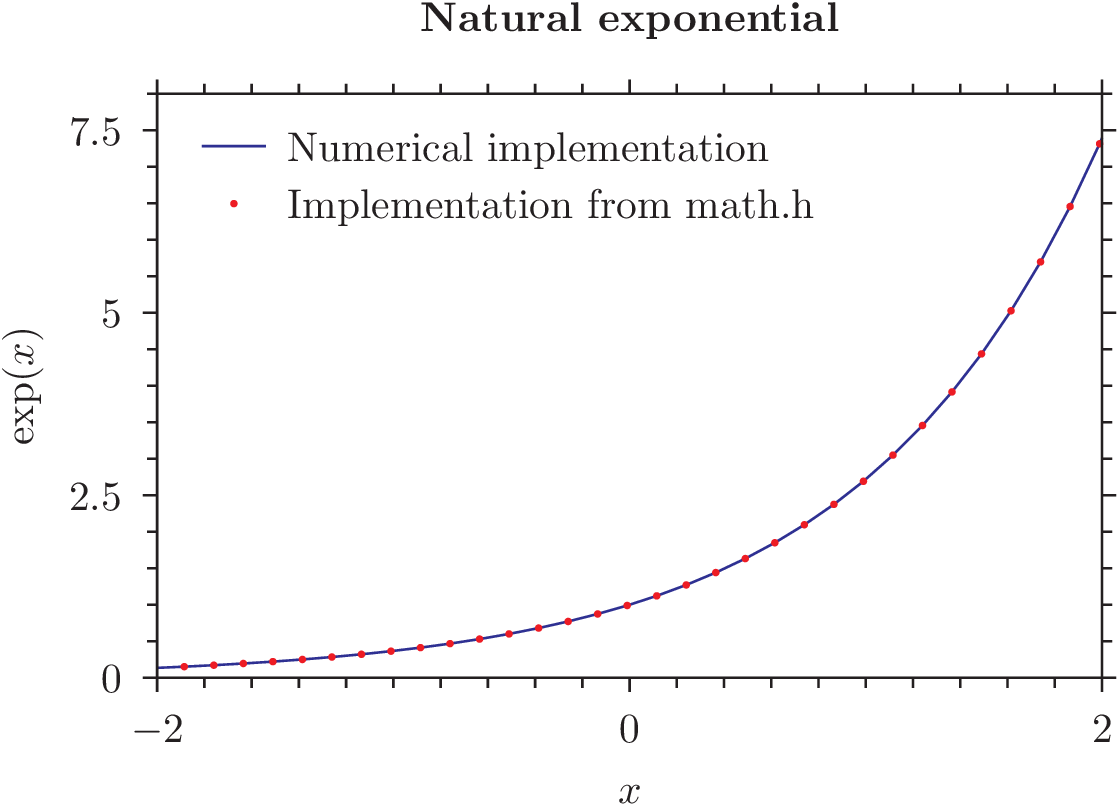
\includegraphics[width = \textwidth]{plot.png}
	\caption{Plot of our numerically implementet exponential function rutine vs. the rutine from math.h for the C-language.}
	\label{fig:plot}
\end{figure}

On Figure \ref{fig:plot}, a plot of our numerical implementation is presented alongside a build-in exponential function rutine from math.h.



\end{document}

%%%%%%%%%%%%%%%%%%%%%%%%%%%%%%%%%%%%%%%%%%%%%%%%%%%%%%%%%%%%%%%%%%%%%%%%%%
